\graphicspath{{./assets/}}
\setcounter{mtc}{2}
\chapter{Requirement analysis  }
\fancyhead[R]{\ungaramond\small\textbf{Chaptre 2: Requirement analysis  }}
\minitoc
\newpage
\section*{Introduction}
In this chapter, our analysis is aimed at identifying the key actors in our design, the functional and non-functional needs our system is to provide for. We will then move on to an overview of the sprint bursts we have realized. Finally, we will provide a dissection of the ecosystem in the form of various UML diagrams.
\section{Capturing requirements}
\subsection{Identifying key actors}
In this context, an actor is a user or any other system that interacts with the subject by exchanging signals and data.
\paragraph{Cloud architecture related actors:}
In order to have a devSecOPS compliant approach, it needs to be built on top of a containerized, highly available cloud infrastructure:
\newline
-	Cloud architect: He is responsible for designing and implementing cloud computing solutions.
\newline
-	IaC tools: Although being a piece of software, it is necessary in order to automate provisioning and configuration of resources.
\newline
-	Cloud provider: Usually a third-party entity that allows for elastically allocating resources.
\newline
-	DevSecOPS team: A devSecOPS engineer is the consumer in this case, he uses the provisioned resources to build an ecosystem that is compliant with organizational needs.
\paragraph{CI/CD related actors:}
The cloud resources hold the value of a tool that is then leveraged to assist the development process:
\newline
-	DevSecOPS team: uses the provisioned resources and follows an agile devSecOPS approach to build an ecosystem that is compliant with organizational needs.
\newline
-	Developer: A consumer of the devSecOPS ecosystem as well as the CI/CD workflow.
\newline
-	Company client: He is the end user and provides the specifications on software development.

\subsection{Functional requirements}

Formulating an understanding on functional requirements is a primordial phase in the implementation of the subject.
\newline
-	A cloud-based infrastructure capable of hosting the devSecOPS ecosystem in terms of compute resources, storage and networking.
\newline
-	A continuous integration platform : The desired goal is to provide a CI workflow that channels the development effort in order to continuously ensure code quality.
\newline
-	A CD workflow: provide an automated and continuous delivery and deployment process.

\subsection{Non-functional requirements}
\begin{itemize}[label=\textbullet,font=\normalsize]
\addtolength{\itemindent}{1cm}
\item High availability and resilience: Typically satisfied by distributed backend resources, orchestration and load balancing of workloads. 
\item Performance and scalability: Usually dependent on the cloud provider as well as the used technologies.
\item Security: An inbuilt quality that cloud and DevSecOPS offer by design.
\item Observability: A highly achievable need due the pluggability of containerized environments.
\item Usability: A somewhat hard to achieve requirement due to the rarity of a technologically adept workforce. 
\item Relatively low cost : the need to prioritize self-hosting and adopting opensource alternatives.
\end{itemize}
\newpage
\section{Product backlog }

\subsection{Backlog history }

\begin{longtable}[!ht]{|m{1cm}|m{3cm}|m{1cm}|m{7cm}|m{1.2cm}|}
\hline
 {\textbf{Epic ID}} & {\textbf{EPIC}} & {\textbf{Story ID}} & {\textbf{Story}} & {\textbf{Prior-ity}} \\
 \hline
0 & \raggedright Certified devSecOps training &	0.1 &	Managing and running custom VMs. & \\
\cline{3-5}
&   & 0.2 &	Managing docker containers.	& \\
\cline{3-5}
&   & 0.3 &	CI/CD pipelines. & \\
\hline
1 & Maintenance and cleanup. &	1.1	& Exploring existing infrastructure and resources. & \\
\cline{3-5}
&   &	1.2 & Performing maintenance on enterprise assets. & \\

\hline
2 & Cloud design &	2.1 &	Information gathering phase. & \\
\hline
3 & Resource provisioning &	3.1 &	Provisioning resources using IaC playbooks. & \\
\hline
4 & Infrastructure setup. &	4.1 &	Infrastructure setup using IaC playbooks. & \\
\hline
5 & \raggedright Initial PaaS setup. &	5.1 &	Setting up ingress controller and TLS certificate provisioner.	 & \\
\cline{3-5}
&   & 5.2 &	Setting distributed storage backend.	 & \\
\cline{3-5}
&   & 5.3 &	Setting up network load balancer.	 & \\
  \hline
6 & Deployment of CI/CD platform &	6.1 &	Setting up personalized CI/CD orchestrator.	 & \\
\cline{3-5}
&   & 6.2 &	Setting up quality gate (CI).	 & \\
\cline{3-5}
&   & 6.3 & Setting up CD controller.	 & \\
  \hline
7 & \raggedright Preparation of automated CICD workflows. &	7.2 &	Structuring SCM backend	 & \\
\cline{3-5}
&   & 7.2 &	 \raggedright Using GitOPS and devOPS tools to automate CI/CD pipelines.	 & \\
   \hline
   \newpage
     \hline
8 & \raggedright Deployment of authentication / authorization backend 	& 8.1 & \raggedright Self-managing distributed database storage backends (redis, mongoDB, postgresql).	 & \\
\cline{3-5}
&   & 8.2 &	\raggedright Deployment and configuration of authentication and authorization services.	 & \\
\cline{3-5}
&   & 8.3 &	\raggedright Configuring forward auth middlewares for secure access.	 & \\
   \hline
9 & \raggedright Implement a resilient disaster recovery strategy. & 9.1 &\raggedright  Provisioning cloud storage resources.		 & \\
\cline{3-5}
&   & 9.2 & \raggedright Preparing and applying backup strategy for application specific data.	 & \\
\cline{3-5}
&   & 9.3 &	\raggedright Preparing and applying backup strategy for PaaS specific workloads.	 & \\
 \hline
% 10	& \raggedright Load testing, benchmarking.& 10.1 & Load testing and benchmarking of assets. & \\	
% \hline

\end{longtable}
% \raggedright for space issue

\newpage
\subsection{Sprint planification }
The project lasted seven months and a half starting on March 1st 2022. Overall, ten sprints have been followed with the typical duration of 3 weeks for each. 


\begin{table}[h!]
\center
\begin{tabular}[b]{|m{2cm}|m{9cm}|m{2cm}|}
\hline
 {\textbf{Sprint ID}} & {\textbf{Sprint Details }} & {\textbf{Duration }} \\ \hline 
0 
&
The first period was spent following a company sponsored devSecOps training. The following elements have been covered: 
Creating vm images using packer, spinning up virtual machines using vagrant,  
Using docker, docker compose plugin and docker container orchestration in swarm, 
An overview on CI/CD pipelines using Jenkins. 
&
4 weeks  \\
\hline
1 
&
The following three weeks were dedicated to exploring the existing infrastructure. Performing some maintenance and planning for migration. 
&
3 weeks  \\ \hline
2 
&
Next, we have started the information gathering phase in which we have formed an initial overview of the desired goals we would like to reach. 
&
2 weeks \\ \hline
3 
&
The use of IaC allowed us to provision the main cloud resources dedicated to hosting the PaaS infrastructure. 
&
2 weeks \\ \hline
4 
&
An initial setup of the provisioned resources was then automated and performed. 
&
3 weeks \\ \hline
5 
&
Putting in place the basic PaaS services, namely a distributed storage backend, a layer 2 load balancer, a cloud-native layer 4 ingress controller to route requests serving also as a reverse proxy and an application load balancer. 
&
3 weeks \\ \hline
6 
&
Mounting the backing CI/CD services which are mostly personalized to company needs. 
&
3 weeks \\ \hline
7 
&
Levering the CI/CD ecosystem to put in place pipelines to automate product testing, code quality checks, and delivery. 
&
4 weeks \\ \hline
8 
&
Securing access to company assets using an Authentication/Authorization middleware. 
&
3 weeks \\ \hline
9 
&
Putting in place a disaster recovery strategy that leverages distributed storage and S3 compliant object storage. 
&
3 weeks \\ \hline
% 10 
% &
% Assessing the performance of the PaaS put in place and planning to enhancements 
% &
% 2 weeks \\ \hline
\end{tabular}
\caption{Table Sprint planification}
\textcolor{white}{I} \label{tab:tab-m}
\end{table}

\newpage
\section{Modeling for cloud architecture and devops }

In order to facilitate collaboration and formulate an understanding of the system specifications and requirements, we have used the Unified Visual Language (UML). 

\subsection{Cloud related diagrams }

% \subsubsection{Package diagram of the underlying cloud resources:}

% \begin{figure}[!ht]\centering
% 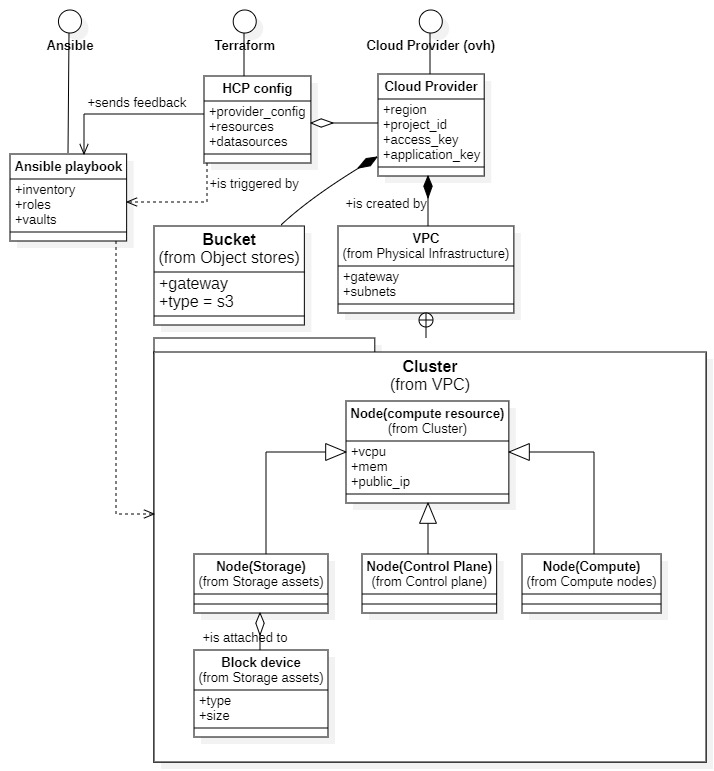
\includegraphics[width=0.8\textwidth,angle=00]{assets/f2.jpg}
% \caption{Package diagram of the underlying cloud resources}
% \label{fig:cloudResrc}
% \end{figure}

% \noindent The cluster resources are basically cloud instances with different specifications tailored to their use cases. Three major groups of resources are distinguished in this diagram : Control plane instances, Compute instances and storage assets which are object store buckets and compute instances to which raw block stores are attached. 

% \newpage
% \subsubsection{Package diagram for the PaaS logical components:}
% \begin{figure}[!ht]\centering
% 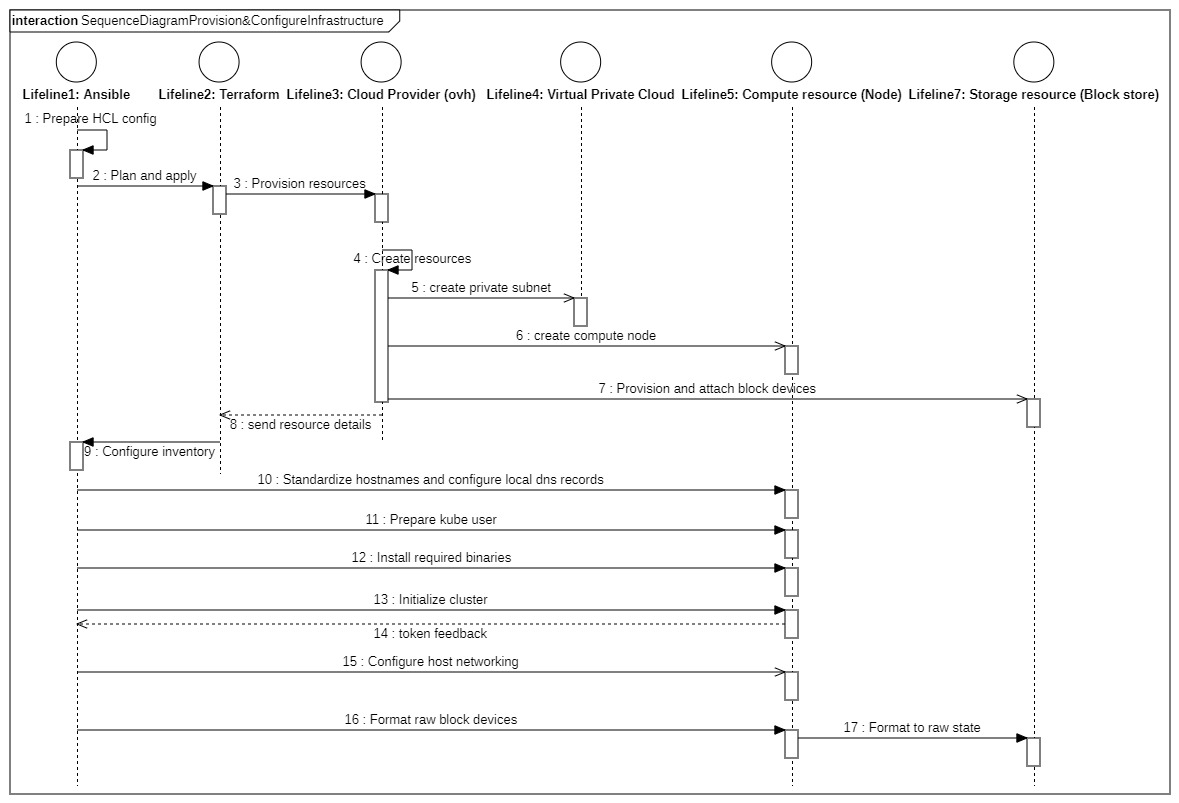
\includegraphics[width=0.8\textwidth,angle=00]{assets/f3.jpg}
% \caption{Package diagram of the underlying cloud resources}
% \label{fig:PaasDiag}
% \end{figure}
% This figure illustrates a package design of the main PaaS services. 

\subsubsection{Class diagram of the provisioned cloud resources:}

\begin{figure}[!ht]\centering
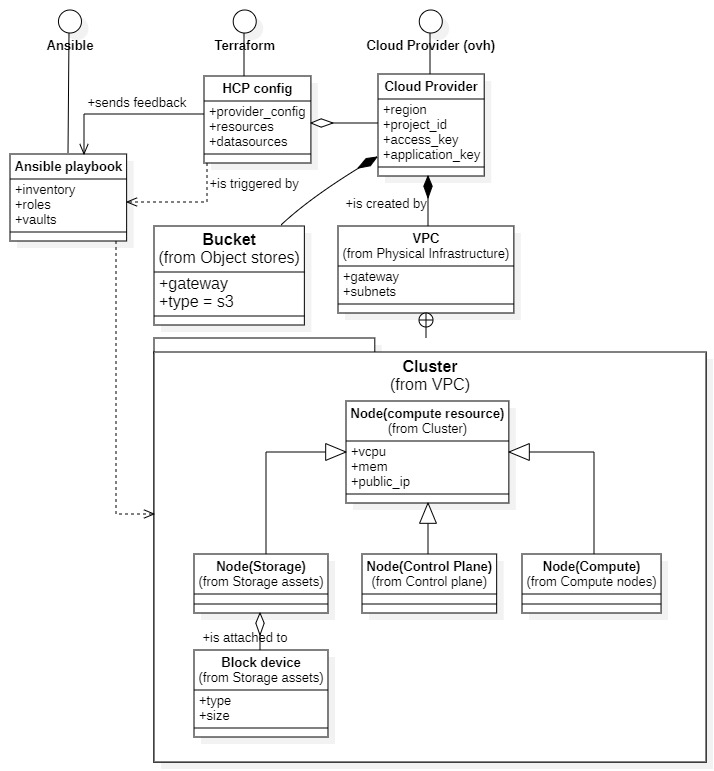
\includegraphics[width=0.8\textwidth,angle=00]{assets/f2.jpg}
\caption{Package diagram of the underlying cloud resources}
\label{fig:f2}
\end{figure}

\subsubsection{Sequence diagram for the provisioning and configuration:}

\begin{figure}[!ht]\centering
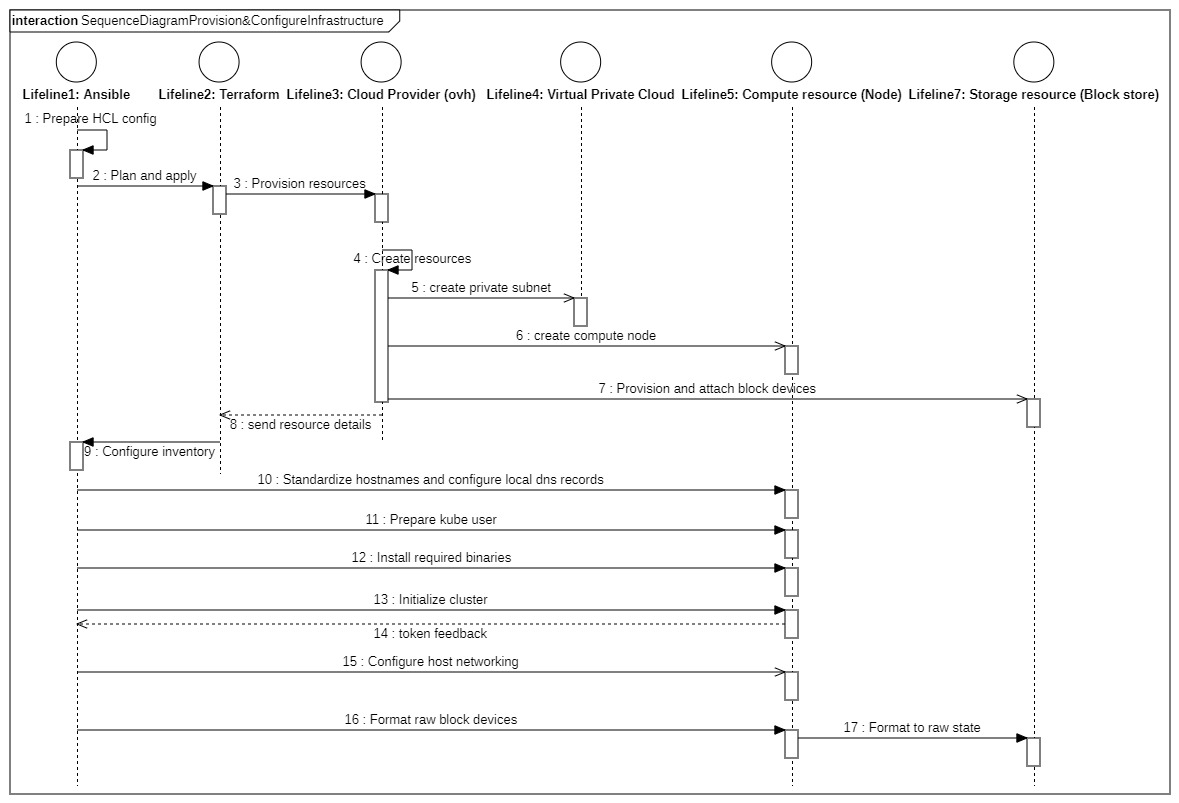
\includegraphics[width=0.8\textwidth,angle=00]{assets/f3.jpg}
\caption{Sequence diagram for the provisioning and configuration}
\label{fig:f3}
\end{figure}

\subsection{CI/CD related diagrams}

\subsubsection{Sequence diagram of a sample deployment: }

\begin{figure}[!ht]\centering
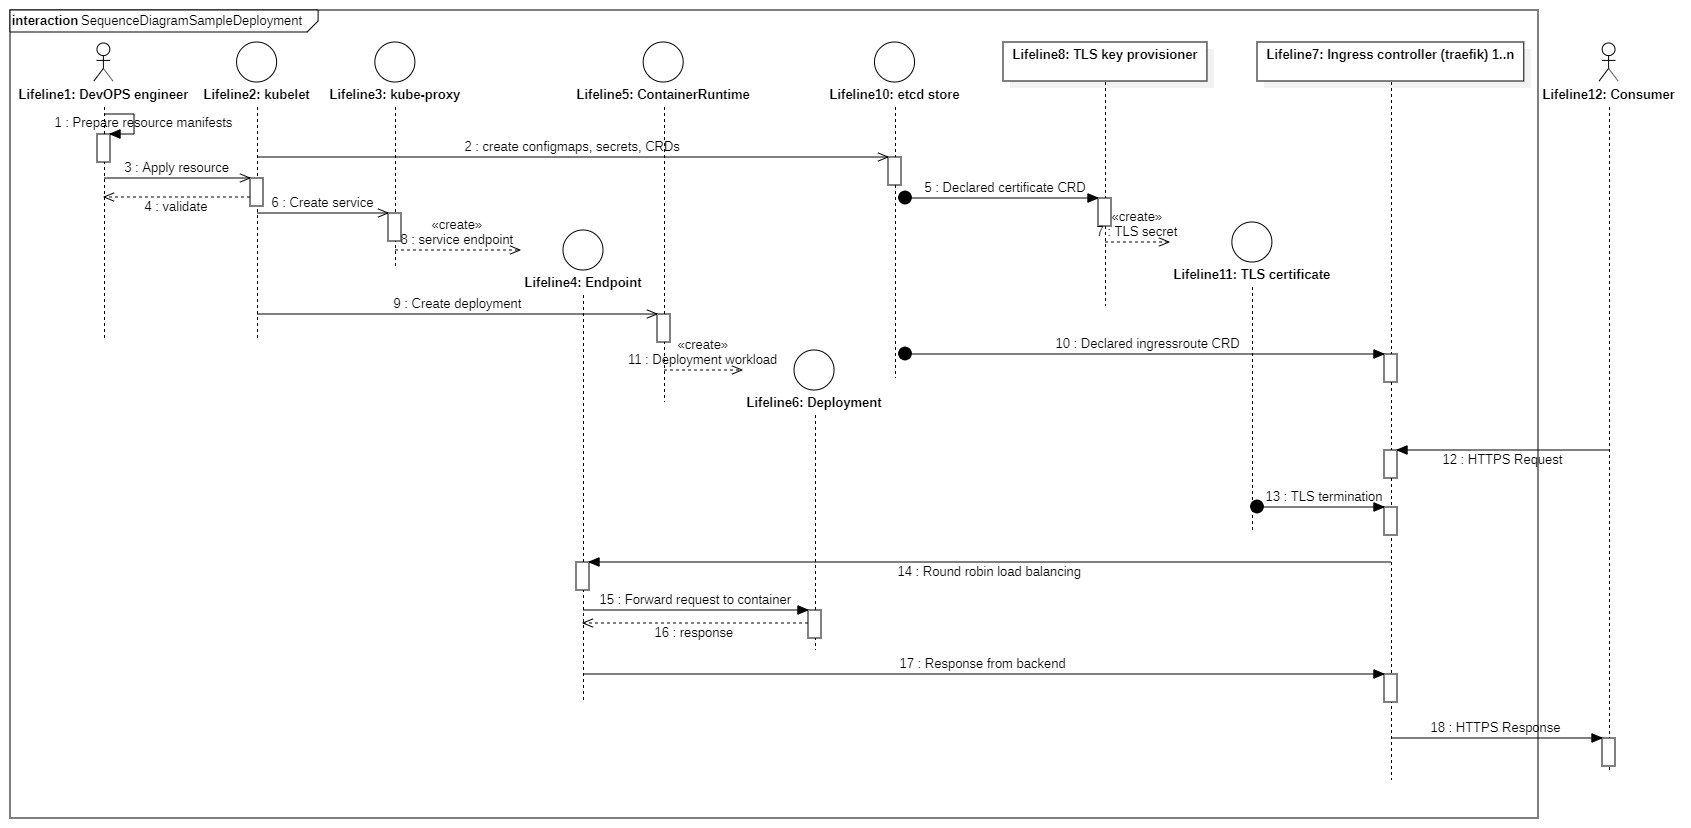
\includegraphics[width=0.8\textwidth,angle=00]{assets/f4.jpg}
\caption{Sequence diagram of a sample deploymen}
\label{fig:f4}
\end{figure}

\newpage 
\subsubsection{Sequence diagrams of the CI/CD workflow: }

\begin{figure}[!ht]\centering
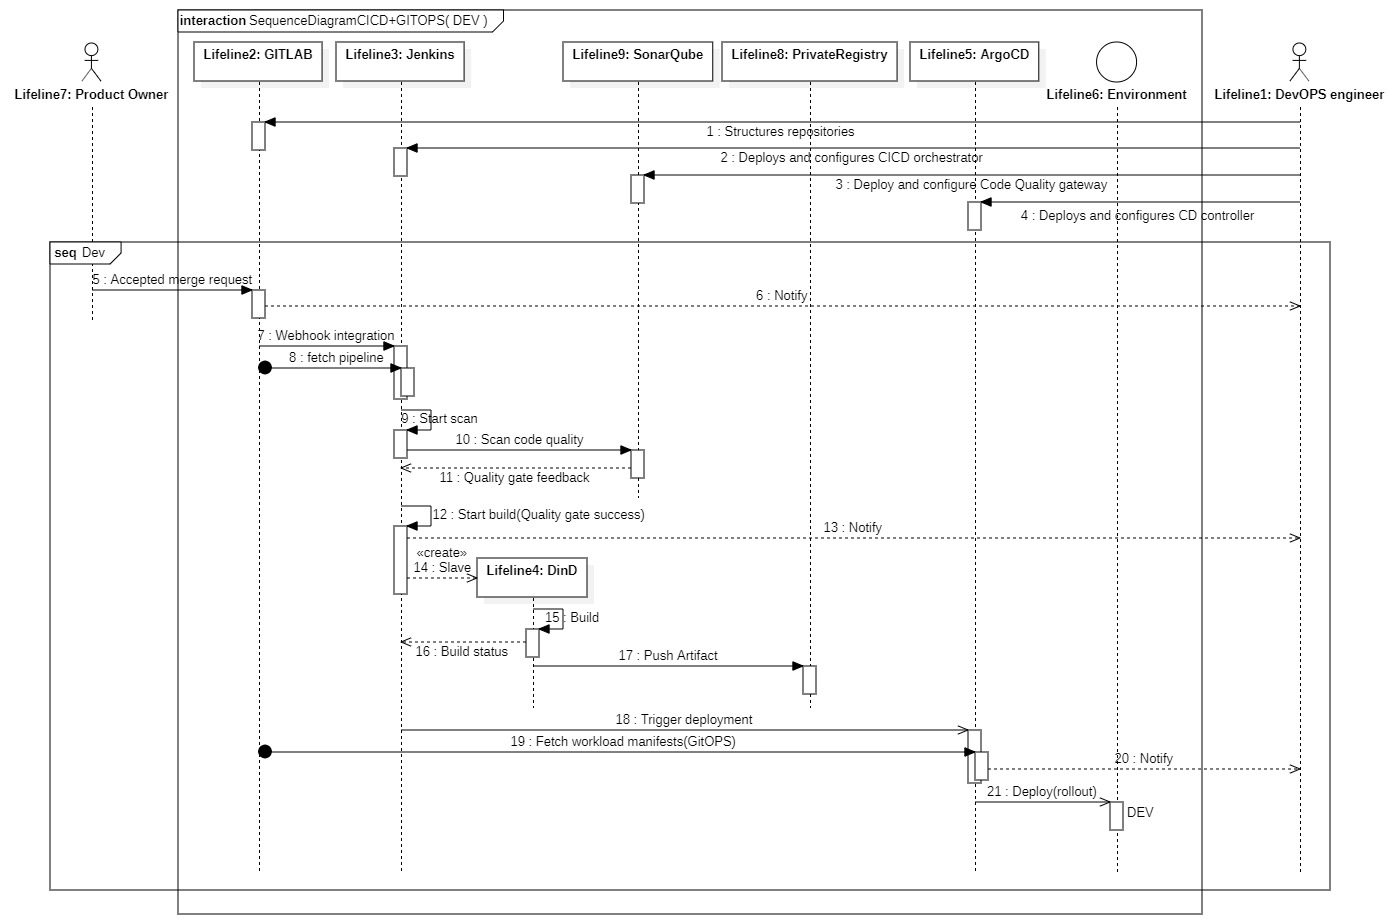
\includegraphics[width=0.8\textwidth,angle=00]{assets/f5.jpg}
\caption{Sequence diagrams of the CI/CD workflow}
\label{fig:f5}
\end{figure}

\begin{figure}[!ht]\centering
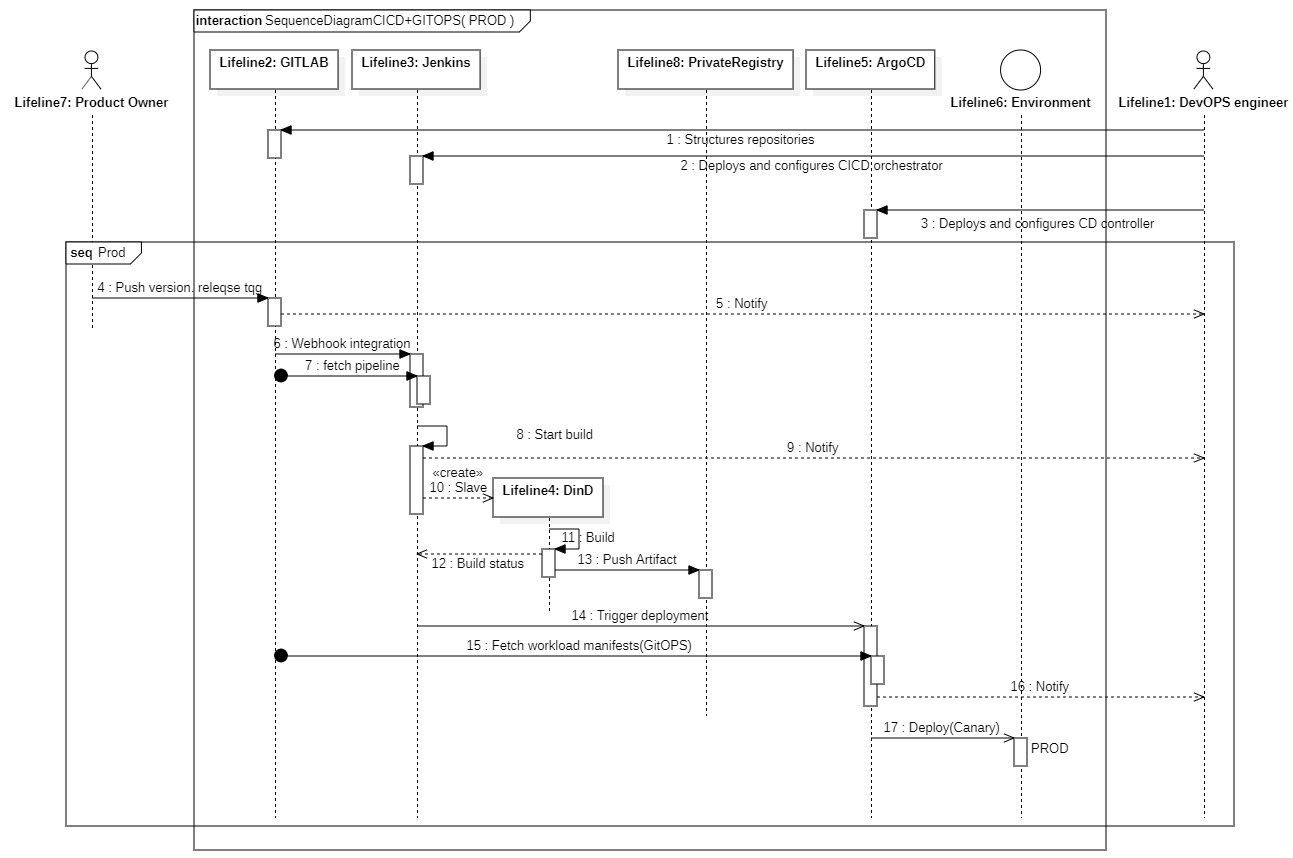
\includegraphics[width=0.8\textwidth,angle=00]{assets/f6.jpg}
\caption{Sequence diagrams of the CI/CD workflow}
\label{fig:f6}
\end{figure}


\newpage
\subsection{Technological choices }
% \paragraph{Development tools }
In this section, we layout the cloud provider choice,
\subsubsection{Cloud provider choice: } 

\paragraph{OVH : }

A decisive factor concerning the cloud provider choice is related to company’s desire to opt mainly for a provider that is based in France.  

\paragraph{Openstack: }

OVH uses openstack as its backing cloud computing infrastructure. Thus, conversing with components as neutron, nova, glance, swift is a must. 

\subsubsection{Infrastructure as code tools }

\paragraph{Terraform: }

An industry standard for conversing with cloud providers in order to provision and configure resources. 

\paragraph{Ansible: }

We have opted for ansible because it’s faster than its alternatives namely chef, and easier to use.  

\subsubsection{Containerization and orchestration techniques: }

\paragraph{Container orchestrator: Kubernetes v1.21 }

An open source container orchestration tool that automates the deployment, scaling, and managing containerized applications. 

\paragraph{Container runtime : containerd }

A daemon for linux that manages the complete container lifecycle. 

\paragraph{Container platform : docker-ce v20.10 }

The container management tool that uses containerd to manage container lifecycles and their underlying abstractions such as volumes and networking.  

\paragraph{Container networking: Calico }

A cloud-native plugin deployment in Kubernetes that uses the CNI API to provide a networking and security solution in the cluster. 

\paragraph{Container platform : docker-ce v20.10 }

The container management tool that uses containerd to manage container lifecycles and their underlying abstractions such as volumes and networking. 

\paragraph{Container networking: Calico }

A cloud-native plugin deployment in Kubernetes that uses the CNI API to provide a networking and security solution in the cluster. 


\subsubsection{Self-hosted PaaS services }

\paragraph{Distributed storage backend: Ceph }

A highly reliable, open source, distributed storage platform offering bloc , filesystem and object storage volumes to be leveraged by the orchestrator. 

\paragraph{Ingress Controller: Traefik ingress controller }

An open-source edge router serving as an ingress controller, a reverse proxy and a load balancer. 

\paragraph{Layer 2 load balancer: MetalLB }

This opensource load balancer provides support for bare metal Kubernetes clusters using standard protocols. 

\paragraph{Private registry: harbor }

An open-source private registry serving as a backend to sore artifacts in a secure manner. 

\paragraph{Database storage (document): Redis, MongoDB }

Database storage in document format is provided by a replicated mongoDB cluster. An in memory redis cluster allows for session storage. 

\paragraph{Database storage (SQL): PostgreSQL }

A PostgreSQL cluster in HA mode coupled with a PGpool middleware to distribute load and control replication. 

\paragraph{Authentication middleware: Authelia }

An open-source portal serving as an authentication and authorization server. It leverages the “forward auth” capability of the ingress controller to regulate access. 

\paragraph{User management: OpenLDAP }

An open-source implementation of the Lightweight Directory Access Protocol that is used to manage organizational user credentials and details. 

\paragraph{SCM tool: Gitlab }

An enterprise solution for source code management and versioning. 

\paragraph{CI/CD orchestration: Jenkins }

An open-source automation server which enables build, test, and deployment processes. 

\paragraph{Quality gate: SonarQube }

An open-source platform that allows for continuous inspection of code quality. 

\paragraph{CD controller: ArgoCD, ArgoRollouts }

An open-source declarative, GitOPS continuous delivery tool for Kubernetes. 

\paragraph{Disaster recovery: Velero }

An open-source tool to safely backup and restore, perform disaster recovery, and migrate Kubernetes cluster resources and persistent volumes. 

\paragraph{Config formats: YAML, TOML, HCP config, JSON }

\subsubsection{Development tools }

\paragraph{Development IDE: VS Code }

A pluggable, lightweight opensource IDE. 

\paragraph{SSH platform: Termius }

A platform that offers port forwarding and secure file transfer over ssh. 

\subsubsection{Development languages }

\paragraph{Scripting: python, shell, groovy }

Shell was used to interface with the linux operating system. For conversing with APIs, an assortment of python scripts were developed to automate various tasks, namely, database backups. Jenkins pipelines and configurations were written in groovy. 

\paragraph{Templating: YTT, jinja2 }

To template various configuration files that are dependent on the deployment environment, we used YTT for YAML/JSON. Jinja2 was the main templating tool for ansible playbooks. 

\newpage

\section{Architectural specifications}

\subsection{Physical architecture}

The following figure is an overview of the infrastructure resource setup:

\begin{figure}[!ht]\centering
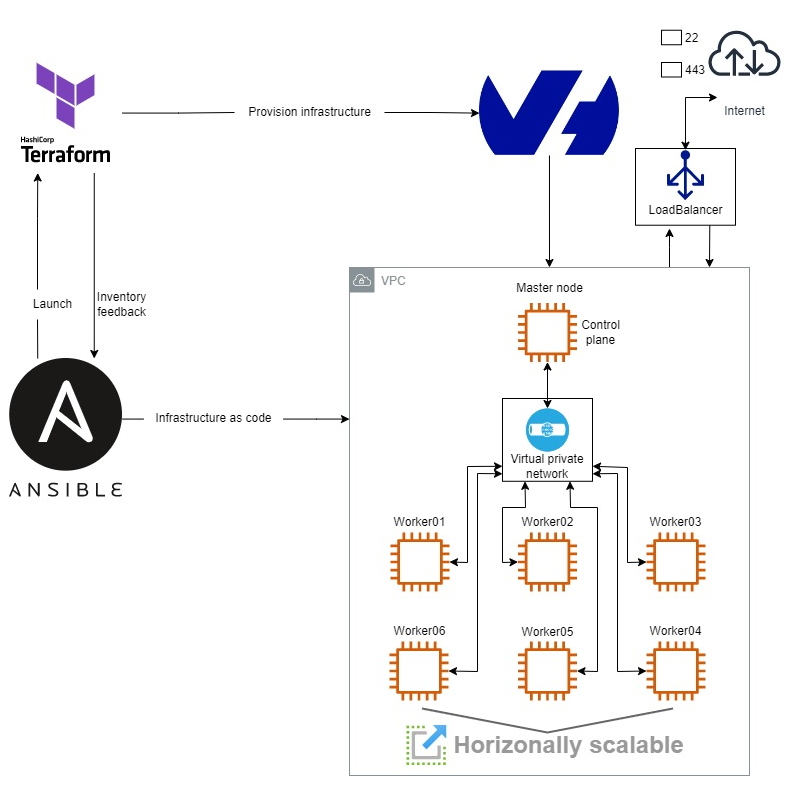
\includegraphics[width=0.8\textwidth,angle=00]{assets/f7.jpg}
\caption{Physical architecture}
\label{fig:f7}
\end{figure}

\newpage

\subsection{PaaS deployment architecture} 
Next we layout the organization of the subsystems, software classes, and layers that make the complete logical system of our PaaS infrastructure :

\begin{figure}[!ht]\centering
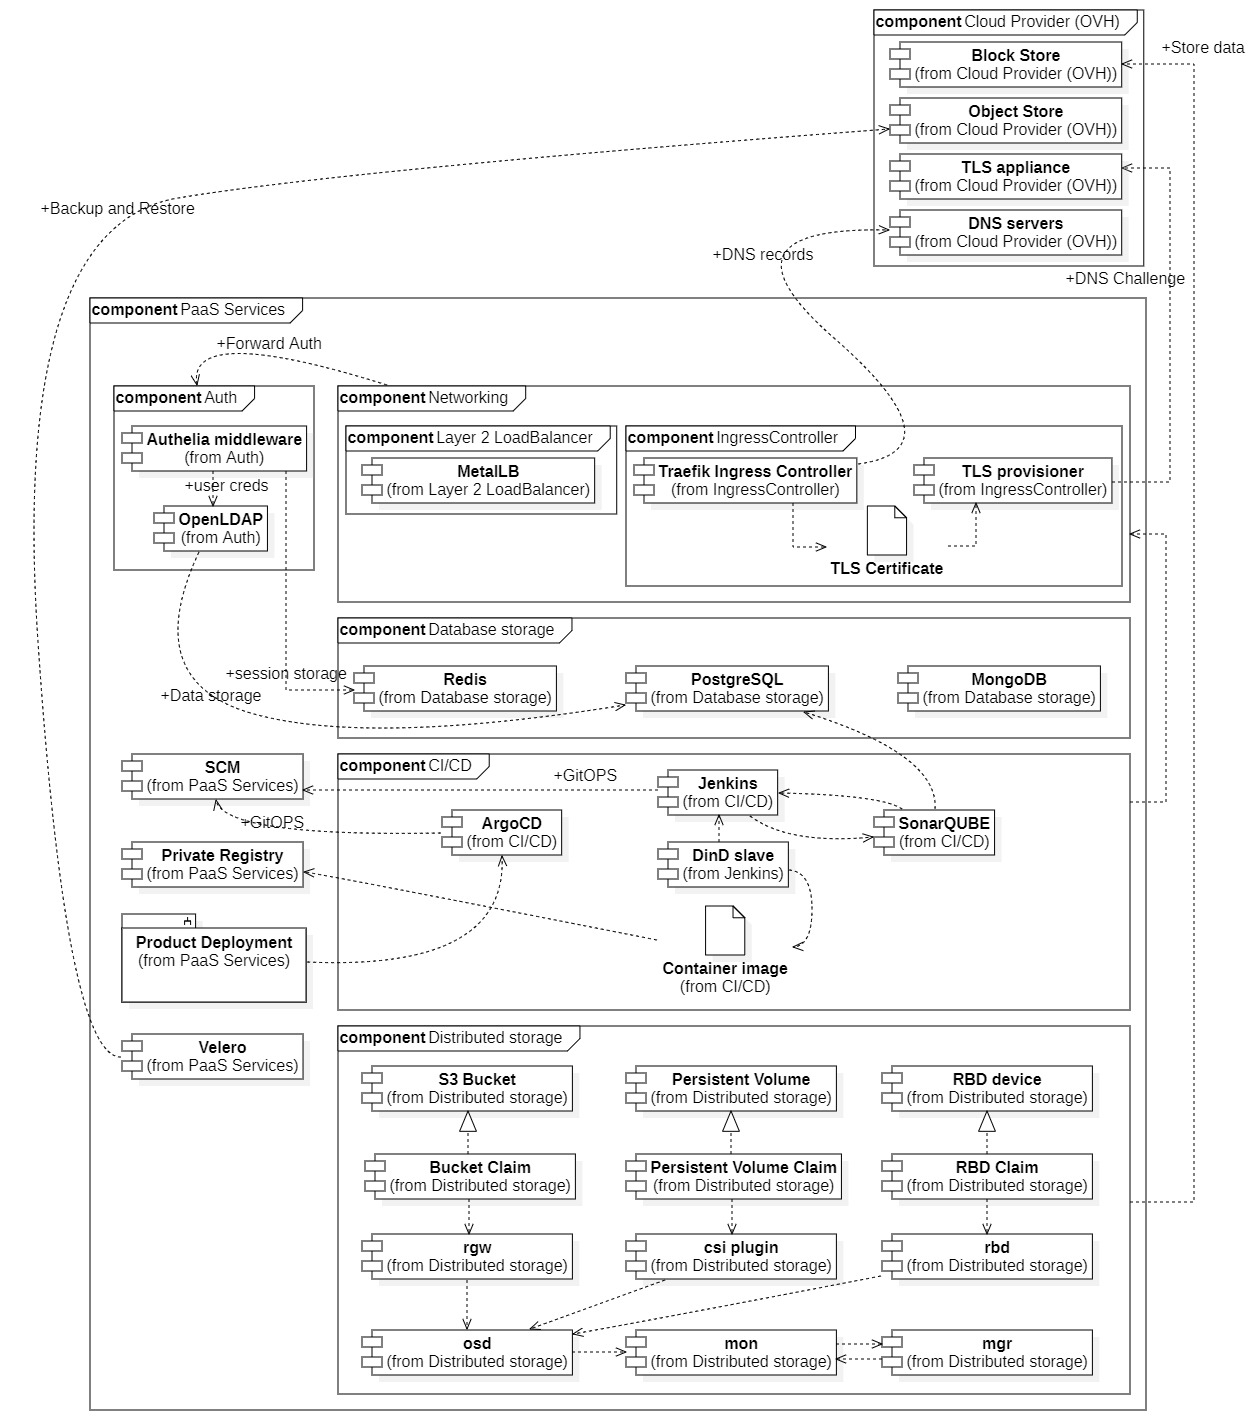
\includegraphics[width=0.8\textwidth,angle=00]{assets/f8.jpg}
\caption{PaaS infrastructure}
\label{fig:f8}
\end{figure}

\section{Workspace description}

To implement the project, the company has provided us with the necessary hardware equipment, certified preliminary training as well as the desired cloud resources.

\section*{Conclusion}
All the functional and non-functional requirements have been viewed in this chapter through the use of package, class and sequence diagrams. We have also formed an understanding on the underlying resources and services through the physical architecture and the PaaS deployment diagram.


% \paragraph{Infrastructure as code tools  }

% \paragraph{Containerization and orchestration techniques  }
% \paragraph{Self-hosted paas services }
% \paragraph{Cloud provider choice}


% \section*{Conclusion}
